\textbf{COLUNI 2020 -- Questão 38}\par\medskip As imagens abaixo correspondem a dois momentos distintos da história dos Estados Unidos. Na primeira delas, nota-se uma manifestação ocorrida na cidade de Chicago, em 2009, acerca da crise econômica que atingia a população americana. Nessa manifestação, destaca-se a utilização de uma célebre fotografia que registrou, no passado, o desalento da população rural americana no contexto da crise econômica de 1929, sobre a qual se lê a frase “salvem nossos lares”. Trata-se da fotografia intitulada “Mãe migrante”, de Dorothea Lange, do ano de 1936, conforme apresentado na imagem II.

\textbf{Imagem I}

% COLUNI-AUTO-FIGURES-BEGIN
\begin{figure}[htbp]
\centering
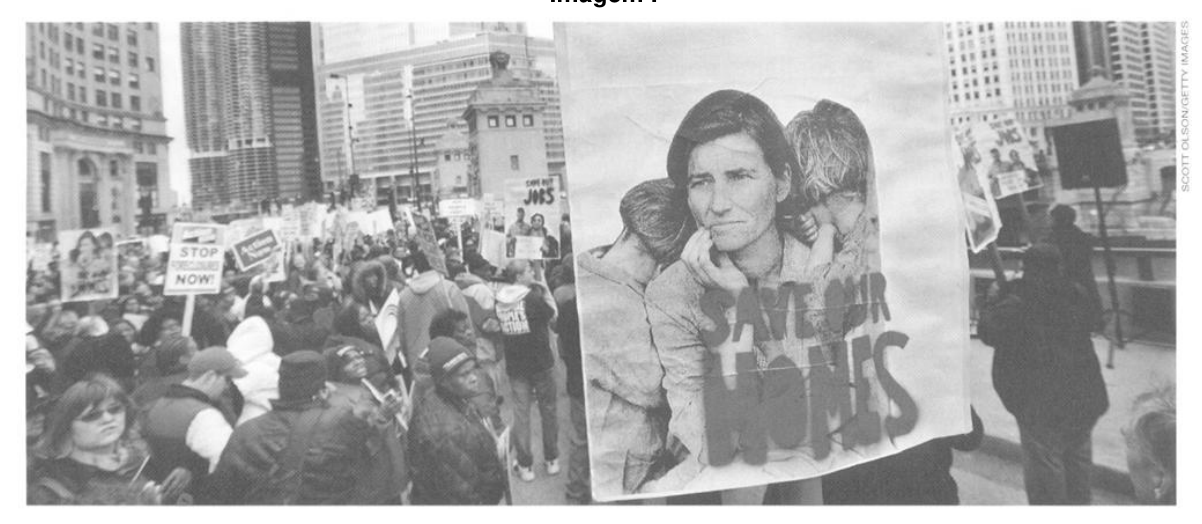
\includegraphics[width=0.95\linewidth]{static/simulados/coluni/figuras/2020/questao-38/figura-1.png}
\end{figure}
% COLUNI-AUTO-FIGURES-END

BRAICK, Patrícia Ramos. \textbf{Estudar História}: das origens do homem à era digital. 2. ed. São Paulo: Moderna, 2015, p. 90.

\textbf{Imagem II}

% COLUNI-AUTO-FIGURES-BEGIN
\begin{figure}[htbp]
\centering
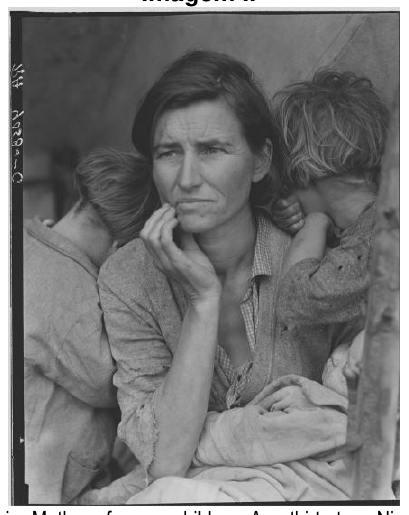
\includegraphics[width=0.95\linewidth]{static/simulados/coluni/figuras/2020/questao-38/figura-2.png}
\end{figure}
% COLUNI-AUTO-FIGURES-END

Dorothea Lange. Destitute pea pickers in California. Mother of seven children. Age thirty-two. Nipomo, California/Migrant Mother. 1936. Library of Congress Prints and Photographs Division, Washington, USA. Disponível em: https://www.loc.gov/item/. Acesso em: 20 set. 2019.

Sobre as semelhanças entre as duas crises econômicas, a de 1929 e a de 2008, é INCORRETO afirmar que:
\begin{enumerate}
\item envolveram uma desregrada especulação no sistema financeiro e causaram impacto no setor produtivo
      dos Estados Unidos.
\item tiveram, como efeitos, a queda da bolsa de valores em âmbito mundial e a rápida repercussão da crise
      econômica em outros países.
\item tiveram, como resultados, danos aos investidores financeiros de outros países e aumento das taxas de
      desemprego nos Estados Unidos.
\item começaram com a declaração de falência de uma tradicional instituição bancária e com a explosão da
      bolha especulativa no setor imobiliário dos Estados Unidos.
\end{enumerate}
